% !TEX root = ../00_thesis.tex

% ------------------------------------------------------------------------------
\section{Single Mode Schedule Synthesis}
\label{sec:single_mode}
% ------------------------------------------------------------------------------
\TTW statically synthesizes the schedule of all tasks, messages, and communication rounds to meet real-time constraints by solving a MILP formulation.
This section presents how to solve it efficiently and ensure that the resulting schedule minimizes the number of communication rounds~\objective{1}.

The schedule of a mode \modeany is computed for one hyperperiod, after which it repeats itself.
To minimize the number of rounds used while handling computational complexity, we solve the problem sequentially, as described in~\cref{alg:outerlayer}.
Each formulation considers a fixed number of rounds $R_{\mode{}}$ to be scheduled, starting with $R_{\mode{}}=0$. The number of rounds is incremented until a feasible solution is found, or until the maximum number of rounds $R_{max}$ (the number of rounds that can ``fit'' into one hyperperiod) is reached.
Thus, \cref{alg:outerlayer} guarantees by construction that if the problem is feasible, the synthesized schedule is optimal in terms of number of rounds used.

\begin{algorithm}
\begin{algorithmic}
\smaller
\Require
	mode \mode{},\;
	$\app \in \mode{}$,\;
	$\tau.\map$,\;
	$\tau.e$, \;
	\nslotsmax, \;
	\Toffset
\Ensure
	\sched{M}

\State $LCM \gets$ \textit{hyperperiod}(\mode{})
\State $R_{max} \gets floor(LCM/\Toffset)$
\State $R_{\mode{}} \gets 0$

\While{$R_{\mode{}} \leq R_{max}$}
	\State formulate the MILP for mode \mode{} using $R_{\mode{}}$ rounds
	\State [ \sched{M}, \textit{feasible} ] = \textit{solve}( MILP )
	\If {\textit{feasible}}
		\Return \sched{M}
	\EndIf
	\State $R_{\mode{}} \gets R_{\mode{}}+1$
\EndWhile
\State \Return 'Problem infeasible'
\end{algorithmic}
\caption{\small Pseudo-code of the single-mode schedule synthesis}
\label{alg:outerlayer}
\end{algorithm}

The MILP formulation contains a set of classical scheduling constraints:
% \begin{itemize}
%
% 	\item
	The precedence constraints between tasks and messages must be respected;
	%
	% \item
	Applications end-to-end deadlines must be satisfied;
	%
	% \item
	Nodes process at most one task simultaneously;
	%
	% \item
	Communication rounds must not overlap;
	%
	% \item
	Rounds must not be allocated more then \nslotsmax messages.
%
% \end{itemize}
These constraints can be easily formulated using our system model (full formulation in \cref{appendix:ttw_artifacts}).
However, one must also guarantee that the allocation of messages to rounds is valid, \ie
\begin{description}
	\item [\constraint{1}]
	Messages must be served in rounds that start after their release time.
	\item [\constraint{2}]
	Messages must be served in rounds that finish before their deadline.
\end{description}
In other word, we must integrate the bin-packing problem of messages to rounds within the MILP formulation.
This is non-trivial and a major difference with the existing approaches for wired architectures~(\eg \cite{craciunas2016Combined}).

To address this challenge, we first formulate the constraints \constraint{1} and \constraint{2} using \emph{arrival}, \emph{demand}, and \emph{service} functions, \af \df and \sf, using network calculus~\cite{leboudec2001Network}.
Those functions count the number of message instances released, with passed deadlines, and served since the beginning of the hyperperiod, respectively.
Those three functions are illustrated in \cref{fig:afdfsf}.
It must hold that
\begin{flalign}
\label{eq:df<sf<af}
&\forall\, m_i \in \messageset, \;\forall\, t,
&&\df_i(t) \leq \sf_i(t) \leq \af_i(t)
&&\\
\label{eq:af_def}
&\text{with},
&&\af_i: \; t \;
	\longmapsto \; \left \lfloor{\frac{t-m_i.o}{m_i.p}}\right \rfloor 	+ 1
	&&\\
\label{eq:df_def}
&\text{and},
&&\df_i: \; t \;
	\longmapsto \; \left \lceil{\frac{t-m_i.o-m_i.d}{m_i.p}}\right \rceil
	&&
\end{flalign}

However, as the service function stays constant between the rounds, we can formulate \constraint{1} and \constraint{2} as follows\\
$\forall\, m_i \in \messageset, \; \forall\, j \in [1 .. R_{\mode{}}], $
\begin{flalign}
\label{eq:af_const}
&\textup{\constraint{1}} \quad  : \quad
	&\sf_i(r_j.t + \Tround) \, &\leq \, \af_i(r_j.t)
	&&
\\
\label{eq:df_const}
&\textup{\constraint{2}} \quad  : \quad
	&\sf_i(r_j.t)  \, &\geq \, \df_i(r_j.t + \Tround)
	&&
\end{flalign}

\begin{figure}
\centering
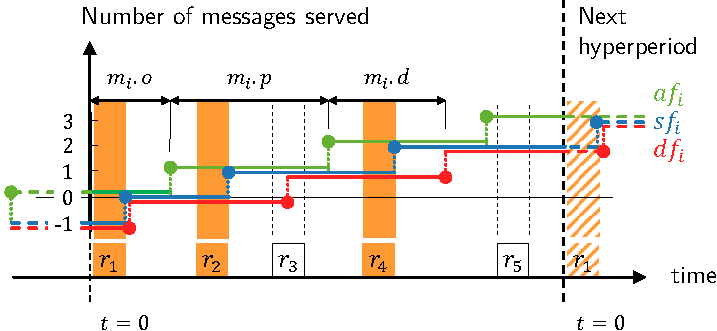
\includegraphics[scale=1]{afdfsf}
\caption{Representation of arrival, demand, and service functions of message $m_i$.
The lower part shows the five round, $r_1$ to $r_5$, scheduled for the hyperperiod.
\capt{%
$m_i$ is allocated a slot in the colored rounds, \ie $r_1$, $r_2$, and $r_4$.
The allocation of $m_i$ to $r_3$ instead of $r_2$ would be invalid, as $r_3$ does not finish before the message deadline, \ie it violates \constraint{2}.
However, the allocation of $m_i$ to $r_5$ instead of $r_1$ would be valid and result in $r_0.B_i = 0$.}
}
\label{fig:afdfsf}
\end{figure}


The arrival and demand functions are step functions. They cannot be used directly in an MILP formulation, however
\begin{flalign}
\label{eq:af=k}
&\forall \; k \in \mathbb{N}, \quad
&&\af_i(t) = k
	\quad \Leftrightarrow \quad
	0 \, \leq \, t - m_i.o - (k-1)m_i.p \,<\, m_i.p &&\\
&\text{and} %\hspace{30pt}
&&\df_i(t) = k
\label{eq:df=k}
	\quad \Leftrightarrow \quad
	0 \, < \, t - m_i.o - m_i.d - (k-1)m_i.p \,\leq\, m_i.p &&
\end{flalign}
For each message $m_i\in \messageset$ and each round $r_j$, $j \in [1..R_{\mode{}}]$, we introduce two integer variables $k^a_{ij}$ and $k^d_{ij}$ that we constraint to take the values of \af and \df at the time points of interest (respectively $r_j.t$ and $r_j.t + \Troundj$). That is,
\begin{align}
\label{eq:ka} %\qquad
0 \, \leq \, r_j.t
	&-m_i.o - (k^a_{ij}-1)m_i.p \,<\, m_i.p\\
\label{eq:kd} %\qquad
0 \, < \, r_j.t
	&+\Troundj - m_i.o - m_i.d - (k^d_{ij}-1)m_i.p \,\leq\, m_i.p\\
\notag
\text{Thus,} \hspace{15pt} &\eqref{eq:ka} \quad \Leftrightarrow  \quad
	 \af_i(r_j.t) = k^a_{ij} \\
\notag
	&\eqref{eq:kd} \quad \Leftrightarrow \quad
	\df_i(r_j.t + \Troundj) = k^d_{ij}
\end{align}

Finally, we must express the service function \sf, which counts the number of message instances served \emph{at the end} of each round.
Remember that $r_k.B_s$ denotes the allocation of the $s$-{th} slot of $r_k$ (\ie the $id$ of the message allocated to the slot).
For any time $t \in \; [ \; r_{j}.t + \Troundj \, ; \,  r_{j+1}.t + \Troundj \; [$, the number of instances of message $m_i$ served is
\begin{align*}
	\sum_{\substack{k = 1}}^{j} \;\;
	\sum_{\substack{s = 1}}^{B}
	 \; r_k.B_s
	 \quad s.t. \; B_s = i
\end{align*}

It may be that $m.o + m.d > m.p$, resulting in $\df(0)=-1$ (\cref{eq:df_def}), like it is the case in \cref{fig:afdfsf}. This ``means'' that a message released at the each of one hyperperiod will have its deadline in the \emph{next} hyperperiod.
To account for this situation, we introduce, for each message $m_i$, a variable $r_0.B_i$ set to the number of such ``leftover'' message instances at $t=0$. Finally, for each message $m_i \in \messageset$, and  $t \in \; [ \; r_{j}.t + \Troundj \, ; \,  r_{j+1}.t + \Troundj \; [$,
\begin{flalign}
\label{eq:sf_def}
\sf_i: \; t \;
	&\longmapsto \;
	\sum_{\substack{k = 1 \\[2pt]s.t. \; r_k.t + \Troundk \, < \, t}}^{j}\;\;
	\sum_{\substack{s = 1 \\[2pt]s.t. \; B_s = i}}^{B}
	 r_k.B_s - r_0.B_i
\end{flalign}

Ultimately, \constraint{1} and \constraint{2} can be formulated as MILP constraints using \cref{eq:ka,eq:kd}, and the following two equations:
\begin{align}
&
\eqref{eq:af_const}\quad	 \Leftrightarrow
	\quad
	\sum_{k = 1}^j
	\sum_{\substack{s = 1 \\[2pt]s.t. \; B_s = i}}^{B}
	 \; r_k.B_s - r_0.B_i \; \leq\;  k^a_{ij}
\\
&
\eqref{eq:df_const}\quad	 \Leftrightarrow
	\quad
	\sum_{k = 1}^{j-1}
	\sum_{\substack{s = 1 \\[2pt]s.t. \; B_s = i}}^{B} \; r_k.B_s - r_0.B_i
	\; \geq\;
	k^d_{ij}
\end{align}


\fakepar{Objective function}
Within our scheduling framework, the MILP does not need to optimize any objective function. Indeed, we mainly want to minimize of the number of rounds $R$ used in the schedule, which is achieved by incrementally increasing the number of rounds until a valid schedule is found~(\cref{alg:outerlayer}).

However, when considering the multi-mode case~(\cref{sec:multi_mode}), it is beneficial to maximize the message deadlines, as illustrated in \cref{fig:msg_deadline_maximization}.
In a nutshell, it relaxes the constraints that are inherited between different modes, and therefore improve the schedulability of the whole problem.
Concretely, the deadline maximization is achieved by setting the following objective to the MILP solver
\begin{align}
&obj \; = \; \sum_{m_i\in \messageset} \, m_i.d
\end{align}


\begin{figure}
	\begin{subfigure}[t]{.48\linewidth}
	\centering
	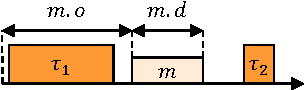
\includegraphics[scale=1]{msg_deadline_base}
	\caption{%
	Example schedule without deadline maximization.
	}
	\label{subfig:msg_deadline_base}
	\end{subfigure}%
	\hfill
	\begin{subfigure}[t]{.48\linewidth}
	\centering
	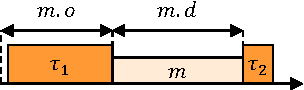
\includegraphics[scale=1]{msg_deadline_maximized}
	\caption{%
	Example schedule with deadline maximization}
	\label{subfig:msg_deadline_maximized}
	\end{subfigure}
	\caption{Illustration of the impact of the message deadlines maximization.
	\capt{%
		If~\cref{subfig:msg_deadline_base} is a valid schedule, then \cref{subfig:msg_deadline_maximized} is also valid, but it
		relaxes the constraints on other modes which also contain message $m$.
		Maximizing the message deadlines improves the schedulability of the multi-mode problem~(\cref{sec:multi_mode}).
	}}
	\label{fig:msg_deadline_maximization}
\end{figure}
